\section{Post-selection inferens}
Klassisk statistisk inferens kan ikke anvendes for adaptive procedurer.
I dette afsnit beskrives teste til inferens efter variabeludvælgelse med en adaptiv metode.
Teorien omkring post-selection inferens er udviklet i nyere tid og er stadig under udvikling.
R-pakkerne \texttt{covTest} og \texttt{selectiveInference} understøtter testene som beskrives i dette afsnit.

\subsection{Kovarians test} \label{subsec:kovarians_test}
I dette afsnit introduceres en test, der tildeler \(p\)-værdier til prædiktorerne valgt af adaptive metoder.
Testen er baseret på LARS algoritmen og blev introduceret af \citep{lockhart}.

Betragt det velkendte lineær regression setup med en responsvariable \(\y \in \mathbb{R}^n\) og en matrix af prædiktorer \(\X \in \mathbb{R}^{n \times p}\), som er relateret ved
\begin{align}
\y = \X \beta + \boldsymbol{\epsilon}, \quad \boldsymbol{\epsilon} \sim N\del{\mathbf{0}, \sigma^2 \mathbf{I}}, \label{eq:set-up}
\end{align}
hvor \(\beta \in \mathbb{R}^p\) er ukendte koefficienter, som skal estimeres.

For at motivere kovarians testen, vil vi først betragte forward-stepwise regression.
Proceduren udvælger én prædiktor af gangen og vælger den prædiktor således at summen af kvadrerede residualer aftager mest.
Lad \(\text{SSR}_k\) betegne summen af kvadrerede residualer for modellen med \(k\) prædiktorer.
Da kan vi udlede en teststørrelse ved at betragte ændringen i SSR
\begin{align*}
R_k = \frac{1}{\sigma^2} \del{\text{SSR}_{k-1} - \text{SSR}_k},
\end{align*}
hvor \(\sigma\) antages at være kendt. 
Denne teststørrelse følger en \(\chi_1^2\) fordeling.
Hvis \(\sigma\) ikke er kendt, da den estimeres udfra sample variansen, hvilket resulterer i en \(F\)-test eller ækvivalent en \(t\)-test til at teste om variabel \(j\) er signifikant.

Betragt forward stepwise regression: start med en tom model, tilføj en prædiktor af gangen, for hvert step vælg den prædiktor \(j\) som giver den største fald i SSR.
Figur \ref{fig:covarians_test}(a) viser kvantilerne for \(R_1\) af forward stepwise regression imod en \(\chi_1^2\) fordeling, hvor \(\beta=0\).
 

%
\begin{figure}[H]
\centering
 \scalebox{0.5}{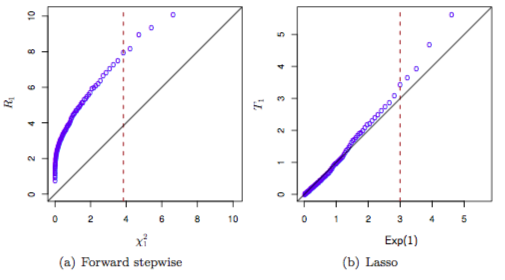
\includegraphics{fig/covarians_test.jpg}}
\caption{Et .}
\label{fig:covarians_test}
\end{figure}
%

Inden vi giver en formel beskrivelse af kovarians testen, gives en betingelse for model matricen \(\X\).
\begin{defn}
Kolonnerne \(\mathbf{X}_1, \ldots, \mathbf{X}_p\) siges at være i generel position hvis the affine span af enhver \(k+1\) vektorer \(s_1 \X_1, \ldots, s_{k+1} \X_{k+1}\) ikke indeholder ethvert element af mængden \(\cbr{\pm \X_i : \ i \neq i_1, \ldots, i_{k+1}}\) for ethvert fortegn \(s_1, \ldots, s_{k+1} \in \cbr{-1,1}\), for \(k < \min \cbr{n,p}\). 
\end{defn}
Ovenstående betingelse er svag og gælder blandt andet når indgangene af \(\X\) kommer af en kontinuert sandsynligheds fordeling.
At kolonnerne af model matrix er i generel position sikre at LARS og lasso stierne er entydig, som vises i \citep{lasso_unique}.

Herefter kan vi defineres teststørrelse af kovarians testen og forklare hvordan \(p\)-værdierne findes.




Lad $\lambda_1 > \lambda_2 > \ldots > \lambda_K$ være knuderne returneret af LARS algoritmen.
Disse er værdierne af regularitets parameteren $\lambda$ ,hvor der sker en ændring i mængden af aktive prædiktorer.
V ønsker, at teste om prædiktoren valgt i \(\lambda_k\) af LARS algoritmen er signifikant.
Lad \(\mathcal{A}_{k-1}\) være den aktive mængde, som består af prædiktorerne med ikke-nul koefficienter, inden denne prædiktor er tilføjet og lad estimatet til slut af dette step være \(\hat{\beta} \del{\lambda_{k+1}}\).
Lad \(\hat{\beta}_{\mathcal{A}_{k-1}} \del{\lambda_{k+1}}\) være løsningen af lasso problemet ved blot at anvende prædiktorerne  i \(\mathcal{A}_{k-1}\), i \(\lambda=\lambda_{k+1}\).
Kovarians teststørrelsen er da defineret ved
\begin{align}
T_k^\text{cov} = \frac{1}{\sigma^2} \del{ \left\langle \y, \X \hat{\beta} \del{\lambda_{k+1}} \right\rangle - \left\langle  \y, \X \hat{\beta}_{\mathcal{A}_{k-1}} \del{\lambda_{k+1}} \right\rangle}. \label{eq:6.5}
\end{align}
Teststørrelsen måler hvor stor en andel af kovariansen mellem outcome og den fittede model som kan tilskrives prediktoren som netop er tilføjet til modellen, dvs forbedringen over intervallet \(\del{\lambda_k, \lambda_{k+1}}\).

Under nulhypotesen at alle $k-1$ variable er i modellen, og under generelle betingelser for modelmatricen $\X$, gælder der for prediktoren i næste trin at
\begin{align*}
T_k^\text{cov} \overset{d}{\rightarrow} \text{Exp}\del{1}
\end{align*}
når \(n, p \rightarrow \infty\).
Når \(\sigma^2\) er ukendt, kan den estimeres under den fulde model \(\hat{\sigma}^2 = \frac{1}{n-p} \text{RSS}_p\). 
Dette indsættes i \eqref{eq:6.5}, og eksponential testen bliver en eksakt \(F_{2,n-p}\) test.

Denne test er også det naturlige analog til degrees of freedom resultaterne for lasso \eqref{eq:df_lasso} og LARS (section 2.5).
Lasso med \(k\) ikke-nul koefficienter forventes at have \(k\) frihedsgrader, og LARS anvender en frihedsgrad for hver segment \(\del{\lambda_{k+1}, \lambda_k}\) langs stien.
Kovarians testen har middelværdi lig en, som er antal frihedsgrader per trin.


Hvis \(\X\) er ortogonal, da er teststørrelsen for kovarians testen givet ved
\begin{align*}
T_k^\text{cov} = \frac{1}{\sigma^2} \lambda_k \del{\lambda_k - \lambda_{k+1}}
\end{align*} 
Derudover fandt vi at \eqref{eq:ortogonal_lasso} som også kan skrives \(\hat{\beta}_j = S_\lambda \del{\frac{1}{n} \mathbf{x}_j^T \y}\).
Lad \(\mathbf{U}_j = \mathbf{x}_j^T \y\) for \(j=1,\ldots, p\). 
Knots i lasso stien er blot værdierne af \(\lambda\) for hvilket koefficienterne er ikke-nul
\begin{align*}
\lambda_1 = \vert \mathbf{U}_{(1)} \vert, \quad \lambda_2 = \vert \mathbf{U}_{(2)} \vert, \quad \ldots, \lambda_p = \vert \mathbf{U}_{(p)} \vert, \quad,
\end{align*}
hvor \(\vert \mathbf{U}_{(1)} \vert \geq \vert \mathbf{U}_{(2)} \vert \geq \dots \geq \vert \mathbf{U}_{(p)} \vert\) er order statistics af \(\vert \mathbf{U}_1 \vert, \ldots, \vert \mathbf{U}_p \vert\).
Derfor 
\begin{align*}
T_k^\text{cov} = \frac{1}{\sigma^2}  \vert \mathbf{U}_{(k)} \vert \del{ \vert \mathbf{U}_{(k)} \vert -  \vert \mathbf{U}_{(k+1)} \vert}
\end{align*}


Kovarians testen har nogle begrænsninger.
Først skal der gælde en betingelse for model matricen \(\X\).
Hvis der eksisterer en kategorisk variabel blandt prædiktorerne, og den resulterende variabel beskrives af dummy variable, da er antagelse om at kolonnerne af \(\X\) er i general position altså ikke overholdt.
Derudover tager testen ikke højde for, hvis nogle variable medtages i modellen mere end én gang (som er tilladt for lasso modificeringen af LARS algoritmen), da behandles hver situation separat og testene udføres separat.
Til sidst er testen kun asymptotisk.

I næste afsnit introduceres en test som kan anvendes efter modeludvælgelse og som giver en eksakt fordeling af teststørrelsen.

\newpage
\subsection{Teste baseret på polyhedral lemmaet}
I dette afsnit introduceres \textit{TG testen}, hvor TG står for "truncated gaussian" og \textit{spacing testen}, som er baseret på polyhedral lemmaet. 
Afsnit er baseret på \citep{post_inference}.
Testene kan anvendes for enhver modeludvælgelses procedure for hvilket udvælgelsen kan karakteriseres ved en mængde af lineære uligheder i \(\y\): \(\cbr{\Gamma \y \geq u}\), hvor \(\Gamma \in \mathbb{R}^{m \times n}\) og \(u \in \mathbb{R}^m\). Uligheden skal fortolkes elementvis.
Den resulterende fordeling af teststørrelsen er eksakt og generelt antager TG testen ingen betingelser på model matricen \(\X\) som er tilfældet for kovarians testen.
Spacing testen er en eksakt version af kovarians testen. 

Antag \(\y \sim N(\tmu, \Sigma)\), hvor \(\tmu \in \R^{n}\) er ukendt, men \(\Sigma \in \R^{n \times n}\) er kendt.
Dette generaliserer set-up i \eqref{eq:set-up}, hvor vi nu tillader en generel fejl kovarians matrix.
For et fast \(\teta \in \R^n\) ønsker vi at lave inferens af \(\teta^T \tmu\) betinget \(\cbr{\Gamma \y \geq u}\).

Nedenfor gives en alternativ repræsentation af polyhedronet.


Indledningsvis introduceres notation som anvendes i dette afsnit.
Vi anvender \(P_L\) for projektions operatoren på det lineære underrum \(L\).
\(\mathbb{P}_{\teta^T \tmu = 0} \del{\cdot \given y \in \mathcal{P}} \) er sandsynligheds målet under \(\tmu\) for hvilket \(\teta^T \tmu =0 \) betinget \(\y \in \mathcal{P}\).
Vi skriver \(\del{M^T M}^+\) for Moore Penrose pseudoinverse af den kvadratiske matrix \(M\) og \(M^+ = \del{M^T M}^+ M^T\) for pseudoinverse af en rektangulær matrix \(M\). 

%Antag \(\y \sim N\del{\boldsymbol{\mu}, \sigma^2 \mathbf{I}_{n \times n}}\) og at vi ønsker at lave inferens betinget på hændelsen \(\cbr{\mathbf{A} \y \leq b}\).
%Mere præcis ønsker vi at lave inferens om \(\boldsymbol{\eta}^T \boldsymbol{\mu}\), hvor \(\boldsymbol{\eta}\) muligvis afhænger af udvægelsen.
%Hvis lasso, LARS .. har udvalgt denne mængde, da kan vi udføre inferens  af de udvalgte variable.
%Vi kunne eventuelt være interesseret i regressions koefficienterne af \(\y\) på \(\X_\mathcal{A}\), dvs \(\hat{\theta}= \del{\X_\mathcal{A}^T \X_\mathcal{A}}^{-1} \X_\mathcal{A}^T \y\).
%Disse svarer til populations parametrene \(\theta= \del{\X_\mathcal{A}^T \X_\mathcal{A}}^{-1} \X_\mathcal{A}^T \boldsymbol{\mu}\), koefficienterne af projectionen af \(\boldsymbol{\mu}\) på \(\X_\mathcal{A}\).
%Dermed kunne \(\boldsymbol{\eta}^T \boldsymbol{\mu}\) svarer til én af disse koefficienter, og dermed er \(\boldsymbol{\eta}\) en af kolonnerne af \(\X_\mathcal{A} \del{\X_\mathcal{A}^T \X_\mathcal{A}}^{-1}\). Dette eksempel fortsættes senere.

%\subsubsection{Conditioning on a single polyhedron}
%Antag \(\y \sim N \del{\boldsymbol{\mu}, \Sigma}\) og \(\boldsymbol{\eta} \in \mathbb{R}^n\) er en potential retning.
%For at forstå fordelingen af
%\begin{align*}
%\boldsymbol{\eta}^T \y \given \cbr{ \mathbf{A} \y \leq b},
%\end{align*}
%kan vi omskrive \(\cbr{\mathbf{A} \y \leq b}\) udfra \(\boldsymbol{\eta}^T \y\) og en komponent \(\mathbf{z}\) som er uafhængig af \(\boldsymbol{\eta}^T \y\). Denne komponent er givet ved
%\begin{align}
%\mathbf{z} = \del{\mathbf{I} - \mathbf{c} \boldsymbol{\eta}^T} \y, \label{eq:z}
%\end{align}
%hvor 
%\begin{align}
%\mathbf{c} = \Sigma \boldsymbol{\eta} \del{\boldsymbol{\eta}^T \Sigma \boldsymbol{\eta}}^{-1}. \label{eq:c}
%\end{align}
%Det ses let, at \(\mathbf{z}\) er ukorreleret og dermed uafhængig af \(\boldsymbol{\eta}^T \y\).
%Hvis \(\Sigma = \sigma^2 \mathbf{I}\), da er \(\mathbf{z}\) blot residualen \(\del{\mathbf{I} - P_{\boldsymbol{\eta}}} \y \) fra projektionen \(\y\) på \(\boldsymbol{\eta}\).
%Vi kan nu omskrive \(\cbr{\mathbf{A} \y \leq b}\) udfra \(\boldsymbol{\eta}^T \y\) og \(\mathbf{z}\).
%
\begin{lem}[Polyhedral lemma] \label{lem:polyhedral}
%Lad \(\mathbf{z}\) være defineret som i \eqref{eq:z} og \(\mathbf{c}\) som i \eqref{eq:c}. 
For ethvert \(\Sigma\) og \(\teta\) således at \(\teta^T \Sigma \teta \neq 0\), da kan \(\cbr{\Gamma \y \geq u}\) udfra \(\teta^T \y\) omskrives til følgende:
\begin{align}
\cbr{\Gamma \y \geq u} \ \Longleftrightarrow \ \cbr{\mathcal{V}^- \del{\y} \leq \boldsymbol{\eta}^T \y \leq \mathcal{V}^+ \del{\y}, \  \mathcal{V}^0 \del{\y} \leq 0}, \label{eq:post_8}
\end{align}
hvor
\begin{align}
\mathcal{V}^- \del{\y} &= \max_{j: \rho_j > 0} \frac{u_j - \del{\Gamma \y}_j + \rho_j \boldsymbol{\eta}^T \y}{\rho_j} \label{eq:V-} \\
\mathcal{V}^+ \del{\y} &= \min_{j: \rho_j < 0} \frac{u_j - \del{\Gamma \y}_j + \rho_j \boldsymbol{\eta}^T \y}{\rho_j} \label{eq:V+} \\
\mathcal{V}^0 \del{\y} &= \max_{j: \rho_j = 0} \del{u_j - \del{\Gamma \y}_j}.  \label{eq:V0} 
\end{align}
og \(\rho=\frac{\Gamma \Sigma \boldsymbol{\eta}}{\teta^T \Sigma \teta}\).
Yderligere  er \(\boldsymbol{\eta}^T \y\) og \(\del{\mathcal{V}^-\del{\y}, \mathcal{V}^+\del{\y},\mathcal{V}^0\del{\y}}\) uafhængige. 
\end{lem}
%\begin{proof}
%Vi kan dekomponere \(\y = \mathbf{c} \del{\boldsymbol{\eta}^T \y} + \mathbf{z}\) og opskrive polyhedronet som følgende
%\begin{align*}
%\cbr{\mathbf{A} \y \leq b} &= \cbr{\mathbf{A} \del{\mathbf{c} \del{\boldsymbol{\eta}^T \y} + \mathbf{z}} \leq b} \\
%&= \cbr{\mathbf{A} \mathbf{c} \del{\boldsymbol{\eta}^T \y} \leq b - \mathbf{A} \mathbf{z} } \\
%&= \cbr{\del{\mathbf{A} \mathbf{c}}_j \del{\boldsymbol{\eta}^T \y} \leq b_j - \del{\mathbf{A} \mathbf{z}}_j \text{ for alle } j} \\
%&= \begin{cases}
%\boldsymbol{\eta}^T \y \leq \frac{b_j - \del{\mathbf{A} \mathbf{z}}_j}{\del{\mathbf{A} \mathbf{c}}_j}, \quad j:\del{\mathbf{A} \mathbf{c}}_j > 0 \\
%\boldsymbol{\eta}^T \y \geq \frac{b_j - \del{\mathbf{A} \mathbf{z}}_j}{\del{\mathbf{A} \mathbf{c}}_j}, \quad j:\del{\mathbf{A} \mathbf{c}}_j < 0 \\
%0 \leq b_j - \del{\mathbf{A} \mathbf{z}}_j, \quad j:\del{\mathbf{A} \mathbf{c}}_j = 0
%\end{cases}.
%\end{align*}
%Da \(\boldsymbol{\eta}^T \y \) er den samme mængde for alle \(j\), må det mindste være maksimum af de nedre grænser, som er \(\mathcal{V}^- \del{\mathbf{z}}\), og ikke mere end minimum af de øvre grænser, som er \(\mathcal{V}^+ \del{\mathbf{z}}\).
%\end{proof}
Resultatet i \eqref{eq:polyhedral} hvor \(\mathcal{V}^-\), \(\mathcal{V}^+\) og \(\mathcal{V}^0\) defineres i \eqref{eq:V-}-\eqref{eq:V0} er deterministisk og gælder for alle \(\y\).
Blot uafhængigheds resultatet afhænger af normaliteten af \(\y\).
Se figur \ref{fig:polyhedron} for en geometrisk illustration af lemmaet.
For simplicitet antages at \(\Sigma= \mathbf{I}\).
Lad os dekomponere \(\y=P_{\boldsymbol{\eta}} \y + P_{\boldsymbol{\eta}^\perp} \y\), hvor \(P_{\boldsymbol{\eta}} \y = \frac{\boldsymbol{\eta} \boldsymbol{\eta}^T \y}{\Vert \boldsymbol{\eta} \Vert_2^2}\) er projektionen af \(\y\) langs \(\boldsymbol{\eta}\) og  \(P_{\boldsymbol{\eta}^\perp} \y = \y - P_{\boldsymbol{\eta}} \y\) er projektionen på ortokomplementet af \(\boldsymbol{\eta}\).
Vi kan betragte \(\y\) som afvigelse fra \(P_{\boldsymbol{\eta}^\perp} \y\) af en mængde \(\boldsymbol{\eta}^T \y\), langs linjen bestemt af \(\boldsymbol{\eta}\).
Mængderne \(\mathcal{V}^-\) og \(\mathcal{V}^+\) betegner hvor langt vi kan afvige fra hver side af \(P_{\boldsymbol{\eta}^\perp} \y\) inden \(\y\) forlader polyhedronen.
Dette giver anledning til uligheden \(\mathcal{V}^- \leq \boldsymbol{\eta}^T \y \leq \mathcal{V}^+\).
Nogle flader af polyhedronen kan være perfekt justeret med \(\boldsymbol{\eta}\), dvs deres normal vektorer kan være ortogonale med \(\boldsymbol{\eta}\).
Dette kan tjekkes udfra \(\mathcal{V}^0\) ved at \(\y\) ligger på den rigtige side af disse flader.  
%--
%Betinget \(P_{\boldsymbol{\eta}^\perp} \y\), ses at hændelsen \(\cbr{\mathbf{A} \y \leq b}\) er ækvivalent med hændelsen \(\mathcal{V}^- \del{\y} \leq \boldsymbol{\eta}^T \y \leq \mathcal{V}^+ \del{\y}\). Yderligere er \(\mathcal{V}^- \del{\y}\) og \(\mathcal{V}^+ \del{\y}\) uafhængige af \(\boldsymbol{\eta}^T \y\), da disse kun er funktioner af \(P_{\boldsymbol{\eta}^\perp} \y\), som er uafhængige af \(\y\).
%--

%
\begin{figure}[H]
\centering
\scalebox{1}{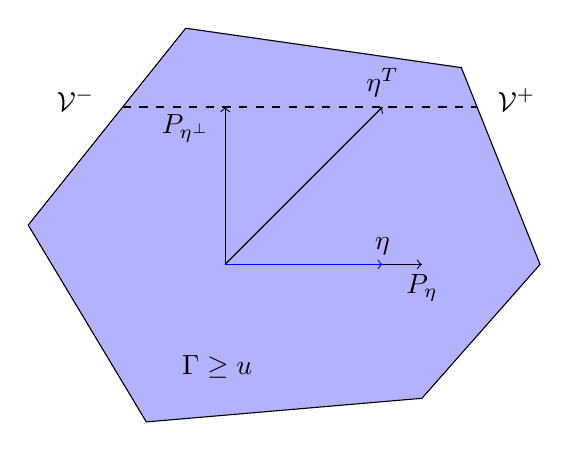
\begin{tikzpicture}
\draw (-1,-2) -- (-2.5,0.5) -- (-0.5,3)-- (3,2.5) -- (4,0) -- (2.5,-1.7) -- (-1,-2)[fill = blue!30];
\draw [<-] (0,2) node [label={[xshift=-0.5cm, yshift=-0.7cm]$P_{\boldsymbol{\eta}^\perp} \y$}] {} -- (0,0);
\draw[<-] (2.5,0) node [below] {$P_{\boldsymbol{\eta}} \y$} -- (0,0);
\draw[<-][blue] (2,0) node [black, above] {$\boldsymbol{\eta}$} -- (0,0);
\draw[<-] (2,2) node [above] {$\boldsymbol{\eta}^T \y$} -- (0,0) node [label={[xshift=1.7cm, yshift=1cm]$\y$}] {};
\draw[dashed] (-1.3,2) node [label={[xshift=-0.6cm, yshift=-0.3cm]$\mathcal{V}^- \del{\y}$}] {} -- (3.2,2) node [label={[xshift=0.5cm, yshift=-0.3cm]$\mathcal{V}^+ \del{\y}$}] {};
\draw node [label={[xshift=-0.1cm, yshift=-1.7cm]$\cbr{\Gamma \y \geq u}$}] {};
\end{tikzpicture}}
\caption{Geometri af polyhedron udvælgelsen som trunkering. For simplicitet antages at \(\Sigma = \mathbf{I}\). Det blå område er polyhedron mængden \(\cbr{\y : \ \Gamma \y \geq u}\).
Ved at opdele \(\y\) til dens projektion på \(\teta\) og dens projektion på det ortogonale komplement af \(\teta\), ser vi at \(\Gamma \y \geq u\) gælder, hvis og kun hvis \(\teta^T \y\) ikke afviger for langt fra \(P_{\boldsymbol{\eta}^\perp} \y\), dvs fastholdt imellem grænserne \(\mathcal{V}^-\) og \(\mathcal{V}^+\).
Yderligere er grænserne \(\mathcal{V}^-\) og \(\mathcal{V}^+\) kun funktioner af \(P_{\boldsymbol{\eta}^\perp} \y\), derfor er de uafhængige af \(\teta^T \y\) under normalitet.} \label{fig:polyhedron}
\end{figure}
%

Af lemma \ref{lem:polyhedral} kan fordelingen af enhver lineær funktion \(\boldsymbol{\eta}^T \y\) betinget \(\Gamma \y \geq u\) skrives som følgende betinget fordeling
\begin{align*}
\boldsymbol{\eta}^T \y \given \mathcal{V}^- \del{\y} \leq \boldsymbol{\eta}^T \y \leq \mathcal{V}^+ \del{\y}, \ \mathcal{V}^0 \del{\y} \leq 0.
\end{align*}
Da \(\boldsymbol{\eta}^T \y\) er normalfordelt, er overstående trunkeret normalfordelt.

En simpel transformation fører til pivotal statistic, som er kritisk for inferens af \(\boldsymbol{\eta}^T \tmu\).

\begin{lem}  \label{lem:lem2}
Lad \(\Phi \del{x}\) betegne fordelingsfunktionen af en standard normalfordeling, da er fordelingsfunktionen for en normalfordeling med middelværdi \(\mu\) og varians \(\sigma^2\) af en stokastisk variable indenfor intervallet \(\sbr{a,b}\) givet ved
\begin{align*}
F_{\mu, \sigma^2}^{\sbr{a,b}} \del{x} = \frac{\Phi\del{\frac{x-\mu}{\sigma}} - \Phi\del{\frac{a-\mu}{\sigma}}}{\Phi\del{\frac{b-\mu}{\sigma}} - \Phi\del{\frac{a-\mu}{\sigma}}}.
\end{align*}
For \(\boldsymbol{\eta}^T \Sigma \boldsymbol{\eta} \neq 0\) da er teststørrelsen \(F_{\boldsymbol{\eta}^T \tmu, \boldsymbol{\eta}^T \Sigma \boldsymbol{\eta}}^{\sbr{\mathcal{V}^-,\mathcal{V}^+}} \del{\boldsymbol{\eta}^T \y} \) a pivotal quantity betinget \(\Gamma \y \geq u\):
\begin{align*}
\mathbb{P} \del{F_{\boldsymbol{\eta}^T \tmu, \boldsymbol{\eta}^T \Sigma \boldsymbol{\eta}}^{\sbr{\mathcal{V}^-,\mathcal{V}^+}} \del{\boldsymbol{\eta}^T \y} \leq \alpha \given \Gamma \y \geq u} = \alpha, 
\end{align*}
for ethvert \(0 \leq \alpha \leq 1\), hvor \(\mathcal{V}^-\) og \(\mathcal{V}^+\) er defineret i \eqref{eq:V-} samt \eqref{eq:V+}. 
\end{lem}
%
Denne pivotal statistic i lemmaet fører til gyldige betinget \(p\)-værdier for at teste nulhypotesen \(H_0: \boldsymbol{\eta}^T \boldsymbol{\mu}=0\) og tilhørende betinget konfidensintervaller for \(\boldsymbol{\eta}^T \tmu\).

%
\begin{lem} \label{lem:lem3}
Givet \(\boldsymbol{\eta}^T \Sigma \boldsymbol{\eta} \neq 0\), antag at vi vil teste
\begin{align*}
H_0: \boldsymbol{\eta}^T \tmu=0 \quad \text{imod} \quad H_1: \boldsymbol{\eta}^T \tmu > 0.
\end{align*}
Definer teststørrelsen
\begin{align}
T=1- F_{0, \boldsymbol{\eta}^T \Sigma \boldsymbol{\eta}}^{\sbr{\mathcal{V}^-, \mathcal{V}^+}} \del{\boldsymbol{\eta}^T \y}, \label{eq:post_1.14}
\end{align}
hvor fordelingsfunktionen af \(\boldsymbol{\eta}^T \y \sim N \del{0,  \boldsymbol{\eta}^T \Sigma \boldsymbol{\eta}}\) i intervallet \(\sbr{\mathcal{V}^-, \mathcal{V}^+}\) er givet i lemma \ref{lem:lem2}.
Da er \(T\) en gyldig \(p\)-værdi for \(H_0\) betinget \(\Gamma \y \geq u\)
\begin{align}
\mathbb{P}_{\boldsymbol{\eta}^T \tmu=0} \del{T \leq \alpha \given \Gamma \y \geq u} = \alpha, \label{eq:post_1.15}
\end{align}
for ethvert \(0 \leq \alpha \leq 1\). 
Definer \(\delta_{\alpha}\) som opfylder, at
\begin{align*}
1-F_{\delta_{\alpha}, \boldsymbol{\eta}^T \Sigma \boldsymbol{\eta}}^{\sbr{\mathcal{V}^- \mathcal{V}^+}} \del{\boldsymbol{\eta}^T \y} &= \alpha.
\end{align*}
Da er \(I= [\delta_\alpha, \infty )\) en gyldig konfidensinterval for \(\teta^T \tmu\) betinget \(\Gamma \y \geq u\)
\begin{align*}
\mathbb{P} \del{\boldsymbol{\eta}^T \tmu \geq \delta_\alpha \given \Gamma \y \geq u} = 1- \alpha.
\end{align*}
\end{lem}
%
TEXT

Nedenfor betragtes en two-sided inferens.
%
\begin{lem} \label{lem:lem4}
Givet \(\boldsymbol{\eta}^T \Sigma \boldsymbol{\eta} \neq 0\), antag at vi vil teste
\begin{align*}
H_0: \boldsymbol{\eta}^T \tmu=0 \quad \text{imod} \quad H_1: \boldsymbol{\eta}^T \tmu \neq 0.
\end{align*}
Definer teststørrelsen
\begin{align}
T=2 \cdot \min\cbr{F_{0, \boldsymbol{\eta}^T \Sigma \boldsymbol{\eta}}^{\sbr{\mathcal{V}^-, \mathcal{V}^+}} \del{\boldsymbol{\eta}^T \y}, 1 - F_{0, \boldsymbol{\eta}^T \Sigma \boldsymbol{\eta}}^{\sbr{\mathcal{V}^-, \mathcal{V}^+}} \del{\boldsymbol{\eta}^T \y}}, \label{eq:post_1.18}
\end{align}
hvor fordelingsfunktionen af \(\boldsymbol{\eta}^T \y \sim N \del{0,  \boldsymbol{\eta}^T \Sigma \boldsymbol{\eta}}\) i intervallet \(\sbr{\mathcal{V}^-, \mathcal{V}^+}\) er givet i lemma \ref{lem:lem2}.
Da er \(T\) en gyldig \(p\)-værdi for \(H_0\) betinget \(\Gamma \y \geq u\)
\begin{align}
\mathbb{P}_{\boldsymbol{\eta}^T \tmu=0} \del{T \leq \alpha \given \Gamma \y \geq u} = \alpha, \label{eq:post_1.19}
\end{align}
for ethvert \(0 \leq \alpha \leq 1\). 
Definer \(\delta_{\frac{\alpha}{2}}, \delta_{1-\frac{\alpha}{2}}\) som opfylder, at
\begin{align*}
1-F_{\delta_{\frac{\alpha}{2}}, \boldsymbol{\eta}^T \Sigma \boldsymbol{\eta}}^{\sbr{\mathcal{V}^- \mathcal{V}^+}} \del{\boldsymbol{\eta}^T \y} &= \frac{\alpha}{2}, \\
1-F_{\delta_{1-\frac{\alpha}{2}}, \boldsymbol{\eta}^T \Sigma \boldsymbol{\eta} }^{\sbr{\mathcal{V}^- \mathcal{V}^+}} \del{\boldsymbol{\eta}^T \y} &= 1-\frac{\alpha}{2}.
\end{align*}
Da gælder, at
\begin{align*}
\mathbb{P} \del{\delta_{\frac{\alpha}{2}} \leq  \boldsymbol{\eta}^T \tmu \leq \delta_{1-\frac{\alpha}{2}} \given \Gamma \y \geq u} = 1- \alpha.
\end{align*}
\end{lem}
%
Teststørrelse i \eqref{eq:post_1.18} defineret som minimum af den trunkerede norma ..
Beviset for dens nulhypotese i \eqref{eq:post_1.19} kommer af, at hvis \(U\) er en standard uniform fordelingen, da er \(2 \cdot \min \cbr{U,1-U}\) også.
Konstruktionen af konfidensintervallet i -- .


Herefter vil vi vise at modeludvælgelses hændelsen for LARS og lasso kan karakteriseres som et polyhedron (dvs kegler) på formen \(\cbr{\y : \ \Gamma \y \geq u}\).

\subsubsection{Polyhedral mængder for LARS udvælgelses hændelse}

Lad os opsummere en kort beskrivelse af stepsene i LARS algoritmen
I step \(k\), initialiseres mængden af aktive variable og listen af fortegn med \(A=\sbr{j_1}\) og \(S_{A_1} = \sbr{s_1}\), hvor \(j_1\) og \(s_1\) opfylder
\begin{align}
\del{j_1, s_1} = \arg \max_{j=1,\ldots, p, \ s \in \sbr{-1,1}} s \mathbf{x}_j \y. \label{eq:polyhedron_rep_LARS1}
\end{align}
Første knot er givet ved
\begin{align*}
\lambda_1 = s_1 \mathbf{x}_{j_1}^T \y.
\end{align*}
For det generelle step \(k > 1\), konstrueres listen \(A_k\) ved at tilføje \(j_k\) til \(A_{k-1}\) og listen \(s_{A_k}\) konstrueres ved at tilføje \(s_k\) til \(s_{A_{k-1}}\), hvor \(j_k\) og \(s_k\) opfylder, at
\begin{align}
\del{j_k, s_k} = \arg \max_{j \notin A_{k-1} , \ s \in \sbr{-1,1}} \frac{\mathbf{x}_j^T P_{A_{k-1}}^\perp \y}{s - \mathbf{x}_j^T \del{\mathbf{x}_{A_{k-1}}^+}^T s_{A_{k-1}}} \cdot \mathbb{1} \cbr{\frac{\mathbf{x}_j^T P_{A_{k-1}}^\perp \y}{s - \mathbf{x}_j^T \del{\mathbf{x}_{A_{k-1}}^+}^T s_{A_{k-1}}} \leq \lambda_{k-1}}, \label{eq:polyhedron_rep_LARS2}
\end{align}
hvor \(P_{A_{k-1}}^\perp \) er projektionen ortogonal med column space af \(\mathbf{X}_{A_{k-1}}\), \(\mathbb{1} \cbr{\cdot}\) er indikator funktionen og \(\lambda_{k-1}\) er knot værdien af step \(k-1\).
Det \(k\)'te knot er da givet ved
\begin{align}
\lambda_k = \frac{\X_{jk}^T P_{A_{k-1}}^\perp \y}{s_k - \X_{jk}^T \del{\X_{A_{k-1}}^+}^T s_{A_{k-1}}}. \label{eq:polyhedron_rap_LARS3}
\end{align}
Algoritmen afsluttes efter \(k\)-step hvis \(k=p\) eller hvis \(\lambda_{k+1} < 0\).

Herefter vil vi verificere at LARS udvælgelses hændelsen
\begin{align}
\mathcal{P} = \cbr{y: \ \hat{A}_k \del{\y} = A_k, \ \hat{s}_{A_k} \del{\y} = s_{A_k}, \ \hat{S}_\ell \del{\y} = S_\ell, \ \ell = 1, \ldots, k} \label{eq:post_28}
\end{align}
er en polyhedron på formen \(\mathcal{P} = \cbr{\y : \ \Gamma \y \geq 0}\).

Polyhedral repræsentationen for \(\mathcal{P}\) i \eqref{eq:polyhedron_rep_LARS} kan bevises vha induktion.
For \(k=1\), finder vi, udfra \eqref{eq:polyhedron_rep_LARS1} at
\begin{align*}
c \del{j_1, s_1}^T \y \geq c \del{j,s}^T \y, \ \forall j \neq j_1, \ s \in \cbr{-1,1},
\end{align*}
hvor \(c \del{j,s} = s \X_j\).
Hermed finder vi, at \(\Gamma\) har \(2 \del{p-1}\) rækker, som er givet ved \(c \del{j_1, s_1} - c \del{j, s}\) for \( \neq j_1, \ s \in \cbr{-1,1}\).
For \(k-1\) step kan optimaliteten af \(j_k\) og \(s_k\) i \eqref{eq:polyhedron_rep_LARS2} udtrykkes som
\begin{align*}
c \del{j_k, s_k, A_{k-1}, s_{A_{k-1}}}^T \y &\geq c \del{j, s, A_{k-1}, s_{A_{k-1}}}^T \y, \ \forall \del{j,s} \in S_k \backslash \cbr{\del{j_k, s_k}}, \\
c \del{j_k, s_k, A_{k-1}, s_{A_{k-1}}}^T \y &\geq 0,
\end{align*}
hvor \(c \del{j, s, A_{k-1}, s_{A_{k-1}}} = \frac{P_{A_{k-1}}^\perp \mathbf{x}_j}{s - \mathbf{x}_j^T \del{\mathbf{x}_{A_{k-1}}^+}^T s_{A_{k-1}}}\).
Mængden \(S_k\) er karakteriseret ved
\begin{align*}
c \del{j, s, A_{k-1}, s_{A_{k-1}}}^T \y &\leq \lambda_{k-1}, \ \del{j,s} \in S_k, \\
c \del{j, s, A_{k-1}, s_{A_{k-1}}}^T \y &\geq \lambda_{k-1}, \ \del{j,s} \in \del{A_{k-1}^c \times \cbr{-1,1}} \backslash S_k.
\end{align*}
Af induktionshypotesen er \(\lambda_{k-1} = c \del{j_{k-1}, s_{k-1}, A_{k-2}, s_{A_{k-2}}}^T \y\) selv en lineær funktion af \(\y\).
Derfor konstrueres \(\Gamma\) ved at tilføje følgende \(\vert S_k \vert + 2 \del{p-k+1}\) rækker til førnævnte matrix: 
\(c \del{j_k, s_k, A_{k-1}, s_{A_{k-1}}} - c \del{j, s, A_{k-1}, s_{A_{k-1}}}\) for \(\del{j,s} \in S_k \backslash \cbr{\del{j_k, s_k}}\) \\
\(c \del{j_k, s_k, A_{k-1}, s_{A_{k-1}}}\) \\
\(c \del{j_{k-1}, s_{k-1}, A_{k-2}, s_{A_{k-2}}}  - c \del{j, s, A_{k-1}, s_{A_{k-1}}}\) for \(\del{j,s} \in S_k\) \\
\(c \del{j, s, A_{k-1}, s_{A_{k-1}}} - c \del{j_{k-1}, s_{k-1}, A_{k-2}, s_{A_{k-2}}}\) for \(\del{j,s} \in \del{A_{k-1}^c \times \cbr{-1,1}} \backslash S_k\) \\
Det totale antal af rækker af \(\Gamma\) i step \(k\) af LARS algoritmen er opadtil begrænset af \(\sum_{\ell=1}^k \del{\vert S_\ell \vert + 2 \del{p - \ell + 1}} \leq 3 pk - 3 \frac{k^2}{2} + 3 \frac{k}{2}\).

\subsubsection{Polyhedral mængder for lasso udvælgelses hændelse}
Ved at introducere et step i LARS algoritmen som fjerner variabler fra den aktive mængde hvis deres koefficientsti  går igennem 0, da kan LARS algoritmen anvendes til at løse lasso.
Lad \(\del{j_k^\text{add}, s_k^\text{add}}\) betegne som indgår i modellen næst som defineret i \eqref{eq:polyhedron_rep_LARS2} og lad \(\lambda_k^\text{add}\) være værdien af \(\lambda\) for hvilket de indgår som defineret i \eqref{eq:polyhedron_rap_LARS3}.
Definer variablerne som forlader modellen herefter
\begin{align*}
j_k^\text{del} = \arg \max_{j \in A_{k-1} \backslash \cbr{j_{k-1}}} \frac{e_j^T \X_{A_{k-1}}^+ \y}{e_j^T \del{\X_{A_{k-1}}^T \X_{A_{k-1}}}^{-1} s_{A_{k-1}}} \cdot \mathbb{1} \cbr{\frac{e_j^T \X_{A_{k-1}}^+ \y}{e_j^T \del{\X_{A_{k-1}}^T \X_{A_{k-1}}}^{-1} s_{A_{k-1}}} \leq \lambda_{k-1}}
\end{align*}
og værdien af \(\lambda\) som forlader modellen
\begin{align*}
\lambda_k^\text{del} = \frac{e_{j_k^\text{del}}^T \X_{A_{k-1}}^+ \y}{e_{j_k^\text{del}}^T \del{\X_{A_{k-1}}^T \X_{A_{k-1}}}^{-1} s_{A_{k-1}}}.
\end{align*}



\subsubsection{TG test}
Givet antallet af step \(k\) og matricen \(\Gamma\) for henholdsvis LARS eller lasso, da kan \(p\)-værdierne og konfidensintervallerne nemt udregnes.
Lad os teste nulhypotesen \(H_0: \ \teta^T \tmu = 0\), hvor \(\teta\) er vilkårlig.

Som specificeret af lemma \ref{lem:polyhedral}, udregnes først mængderne
\begin{align*}
\mathcal{V}^- \del{\y} &= \max_{j: \del{\Gamma \teta}_j > 0} - \del{\Gamma \y}_j \cdot \frac{\Vert \teta \Vert_2^2}{\del{\Gamma \teta}_j} + \teta^T \y, \\
\mathcal{V}^+ \del{\y} &= \min_{j: \del{\Gamma \teta}_j < 0} - \del{\Gamma \y}_j \cdot \frac{\Vert \teta \Vert_2^2}{\del{\Gamma \teta}_j} + \teta^T \y.
\end{align*}
Bemærk at antallet af operation for at udregne \(\mathcal{V}^-\) og \(\mathcal{V}^+\) er \(O \del{mn}\), hvor \(m\) er antallet af række i \(\Gamma\).

For at teste imod en one-sided alternativ \(H_1: \ \teta^T \tmu > 0\),  defineres teststørrelsen
\begin{align*}
T_k^\text{tg}=1- F_{0, \sigma^2 \Vert \boldsymbol{\eta} \Vert_2^2}^{\sbr{\mathcal{V}^-, \mathcal{V}^+}} \del{\boldsymbol{\eta}^T \y} = \frac{\Phi \del{\frac{\mathcal{V}^+}{\sigma \Vert \boldsymbol{\eta} \Vert_2}}-\Phi \del{\frac{\boldsymbol{\eta}^T \y}{\sigma  \Vert \boldsymbol{\eta} \Vert_2}}}{\Phi \del{\frac{\mathcal{V}^+}{\sigma  \Vert \boldsymbol{\eta} \Vert_2}}-\Phi \del{\frac{\mathcal{V}^-}{\sigma \Vert \boldsymbol{\eta} \Vert_2}}}.
\end{align*}
Af lemma \ref{lem:lem3}, giver dette en gyldig \(p\)-værdi betinget udvælgelsen, dvs
\begin{align}
\mathbb{P}_{\boldsymbol{\eta}^T \theta = 0} \del{T_k^\text{tg} \leq \alpha \given \hat{A}_k \del{\y} = A_k, \hat{s}_{A_k} \del{y} = s_{A_k}} = \alpha, \label{eq:post_32}
\end{align}
for ethvert \(0 \leq \alpha \leq 1\).
Lemma \ref{lem:lem3} giver også at et betinget konfidensinterval udledes ved først at udregne \(\delta_\alpha\) som opfylder
\begin{align*}
1-F_{\delta_{\alpha}, \boldsymbol{\eta}^T \Sigma \boldsymbol{\eta}}^{\sbr{\mathcal{V}^- \mathcal{V}^+}} \del{\boldsymbol{\eta}^T \y} &= \alpha.
\end{align*}
Da lader vi \(I_k = [\delta_\alpha, \infty)\), som er en passende betinget coverage, da
\begin{align}
\mathbb{P} \del{\boldsymbol{\eta}^T \theta \in I_k \given \hat{A}_k \del{\y} = A_k, \hat{s}_{A_k} \del{\y} = s_{A_k}} = 1-\alpha. \label{eq:post_33}
\end{align}

For at teste imod en two-sided alternative \(H_1: \ \teta^T \tmu \neq 0\), anvendes istedet teststørrelsen
\begin{align*}
T_k^\text{TG}= 2 \cdot \min \cbr{T_k^{\text{tg}}, 1-T_k^{\text{tg}}}.
\end{align*}
Af lemma \ref{lem:lem4}, fås de samme resultaterne i \eqref{eq:post_32} og \eqref{eq:post_33} men med \(T_k^\text{TG}\) istedet for \(T_k^\text{tg}\) og \(I_k'= \sbr{\delta_{\frac{\alpha}{2}}, \delta{1-\frac{\alpha}{2}}}\) istedet for \(I_k\).

For et signifikant niveau $\alpha$ afvises nulhypotesen hvis \(T^{\text{TG}} \leq \alpha\).



Hvis \(\teta = \del{\X_{A_k}^+}^T e_k\), hvor \(e_k\) er den \(k\)'te enhedsvektor, da kan nulhypotesen \(H_0: \ \teta^T \tmu =0\) omskrives til
\begin{align*}
\boldsymbol{\eta}^T \boldsymbol{\mu} = \mathbf{e}_k^T \X_{A_k}^+ \boldsymbol{\mu} = \mathbf{e}_k^T \del{\X^T \X}^{-1} \X^T \X \boldsymbol{\beta} = \beta_k
\end{align*}
Dvs da svarer nulhypotesen til at teste om \(k\)'te variabel er signifikant.


Nulhypotesen for TG testen er stokastisk, da \(\mathcal{V}^-\) og \(\mathcal{V}^+\) er stokastiske variable ...
TG testen for lasso antager blot en generel position af kolonnerne af \(\X\), som er en svag antagelse.
Testen kan bruges for ethvert fast \(\lambda\) og er eksakt.
\newpage

\subsection{Spacing test}
Som nævnt vil matricerne \(\Gamma\), som udregnes for polyhedron repræsentationerne \(\cbr{\y : \ \Gamma \y \geq 0}\), groft sagt have \(3pk\) rækker efter \(k\) steps for LARS og lasso.
Dette betyder, at matricerne hurtigt ekspanderer og da udregningerne af \(\mathcal{V}^-\) og \(\mathcal{V}^+\) afhænger lineært af antallet af rækker i \(\Gamma\), er disse tunge at beregne.
I dette afsnit udledes en simpel approksimation til polyhedron repræsentationen for LARS, som letter disse udregninger. 
Først introduceres en alternativ karakterisering for LARS udvælgelses hændelsen efter \(k\) step.
%
\begin{lem} \label{lem:post_lem5}
Antag LARS algoritmen producerer en liste af aktive variable \(\mathcal{A}_k\) og fortegn \(s_{\mathcal{A}_k}\) efter \(k\) step.
Definer \(c \del{j, s, \mathcal{A}_{k-1}, s_{\mathcal{A}_{k-1}}} = \frac{P_{\mathcal{A}_{k-1}}^\perp \X_{j}}{s - \X_{j}^T \del{\X_{\mathcal{A}_{k-1}}^+}^T s_{\mathcal{A}_{k-1}}}\), hvor \(\mathcal{A}_0 = s_{\mathcal{A}_0} = \emptyset\) således at \(c \del{j, s, \mathcal{A}_{0}, s_{\mathcal{A}_0}} = c \del{j,s} = s \X_j\).
Betragt følgende betingelser:
\begin{align}
c \del{j_1, s_1, \mathcal{A}_0, s_{\mathcal{A}_0}}^T \y &\geq c \del{j_2, s_2, \mathcal{A}_1, s_{\mathcal{A}_1}}^T \y \geq \dots \nonumber \\
&\geq  c \del{j_k, s_k, \mathcal{A}_{k-1}, s_{\mathcal{A}_{k-1}}}^T \y \geq 0, \label{eq:post_34} \\
c \del{j_k, s_k, \mathcal{A}_{k-1}, s_{\mathcal{A}_{k-1}}}^T \y &\geq M_k^+ \del{j_k, s_k, c \del{j_{k-1}, s_{k-1}, \mathcal{A}_{k-2}, s_{\mathcal{A}_{k-2}}}^T \y}, \label{eq:post_35} \\
c \del{j_\ell, s_\ell, \mathcal{A}_{\ell-1}, s_{\mathcal{A}_{\ell-1}}}^T \y &\leq M_\ell^- \del{j_\ell, s_\ell, c \del{j_{\ell-1}, s_{\ell-1}, \mathcal{A}_{\ell-2}, s_{\mathcal{A}_{\ell-2}}}^T \y}, \ \ell = 1, \ldots, k, \label{eq:post_36} \\
0 &\geq M_\ell^0 \del{j_\ell, s_\ell, c \del{j_{\ell-1}, s_{\ell-1}, \mathcal{A}_{\ell-2}, s_{\mathcal{A}_{\ell-2}}}^T \y}, \ \ell = 1, \ldots, k, \label{eq:post_37} \\
0 &\leq M_\ell^S \y,  \ \ell = 1, \ldots, k. \label{eq:post_38}
\end{align}
For \(\ell = 0\) i \eqref{eq:post_36} og \eqref{eq:post_37} gælder, at \(c \del{j_0, s_0, \mathcal{A}_{-1}, s_{\mathcal{A}_{-1}}}^T \y = \infty\).
Mængden af alle \(\y\) som opfylder ovenstående betingelser er de samme som mængden \(\mathcal{P}\) i \eqref{eq:post_28}.

Der gælder, at mængden \(M_k^+\) i \eqref{eq:post_35} kan skrives som et maksimum af lineære funktioner af \(\y\), at hver \(M_\ell^-\) i \eqref{eq:post_36} kan skrives som et minimum af lineære funktioner af \(\y\), at hver \(M_\ell^0\) i \eqref{eq:post_37} kan skrives som et maksimum af lineære funktioner af \(\y\) og at hver \(M_\ell^S\) i \eqref{eq:post_38} er en matrix.
Dermed kan \eqref{eq:post_34}-\eqref{eq:post_38} udtrykkes som \(\Gamma \y \geq 0\) for en matrix \(\Gamma\).
Antallet af rækker af \(\Gamma\) er opadtil begrænset af \(4pk - 2 k^2 -k\).
\end{lem}
%
Ved første øjekast lader det ikke til, at lemma \ref{lem:post_lem5} giver megen hjælp til polyhedron karakteriseringen i section ---.
Efter \(k\) step har vi nu en matrix \(\Gamma\) som har en orden af \(4pk\) rækker, som faktisk er mere end før.
Men hvis vi ser bort fra betingelserne \eqref{eq:post_36}-\eqref{eq:post_38}, er karakteriseringen i lemma \ref{lem:post_lem5} langt mere kortfattet.

Hvis \(\X\) er ortogonal, da har vi, at \(M_\ell^-= \infty\) og \(M_\ell^0=-\infty\) og matricen \(M_\ell^S\) har nul rækker for hver \(\ell\).
Dette betyder, at betingelserne \eqref{eq:post_36}-\eqref{eq:post_38} er intetsigende.
Polyhedron karakteriseringen i lemma \ref{lem:post_lem5}, reduceres derfor til \(\cbr{\y: \ \Gamma \y \geq U}\), hvor \(\Gamma\) kun har \(k+1\) rækker, defineret ved de \(k+1\) betingelser i \eqref{eq:post_34} og \eqref{eq:post_35} og \(U\) er en stokastisk vektor med komponenterne \(U_1 = \dots = U_k=0\) og \(U_{k+1}= M_k^+ \del{j_k,s_k, c \del{j_{k-1}, s_{k-1}, \mathcal{A}_{k-2}, s_{\mathcal{A}_{k-2}}}^T \y}\).

For en generel ikke-ortogonal matrix \(\X\), kan vi stadig betragte at ignorere betingelserne \eqref{eq:post_36}-\eqref{eq:post_38} og anvende den kompakte repræsentation \(\cbr{\y: \ \Gamma \y \geq U}\) givet ved \eqref{eq:post_34} og \eqref{eq:post_35}.
Dette er en approksimation til den eksakte polyhedron karakterisering i lemma \ref{lem:post_lem5}, men udregningsmæssig mere attraktiv, da \(\Gamma\) kun har \(k+1\) rækker.

Vi vil nu anvende teorien til \(\cbr{\y: \ \Gamma \y \geq U}\).
Da ækvivalensen  i \eqref{eq:post_8} er et deterministisk resultat, gælder det også for et stokastisk \(U\).
Men uafhængigheden mellem \(\boldsymbol{\eta}^T \y\) og \(\del{\mathcal{V}^-\del{\y, U}, \mathcal{V}^+\del{\y, U},\mathcal{V}^0\del{\y, U}}\) er ikke umiddelbart opfyldt.
Antag \(\y\) og \(U\) er stokastiske og at
\begin{align}
U \text{ er en funktion af } \del{\mathbf{I}-\Sigma \teta \teta^T / \teta^T \Sigma \teta} \y, \label{eq:post_39}
\end{align}
da er \(\boldsymbol{\eta}^T \y\) og \(\del{ \del{\mathbf{I}-\Sigma \teta \teta^T / \teta^T \Sigma \teta} \y, U }\) uafhængig. 
Da er  \(\boldsymbol{\eta}^T \y\) og \(\del{\mathcal{V}^-\del{\y, U}, \mathcal{V}^+\del{\y, U},\mathcal{V}^0\del{\y, U}}\) uafhængige.
Det kan vises, at betingelsen \eqref{eq:post_39} gælder under milde antagelser af \(\teta\).
Vektoren skal lægge i kolonne space af LARS aktive variable i det nuværende step, dvs \(\teta \in \text{col} \del{\X_{\mathcal{A}_k}}\).

%
\begin{lem}
Antag LARS algoritmen har gennemløbet \(k\) step, og repræsenter betingelserne \eqref{eq:post_34} og \eqref{eq:post_35} i lemma \ref{lem:post_lem5} som \(\Gamma \y \geq U\).
Hvis \(\teta \in \text{col} \del{\X_{\mathcal{A}_k}}\), da gælder betingelsen i \eqref{eq:post_39}, derfor kan inferens for \(\teta^T \tmu\) udføres med redskaberne beskrevet i afsnit --- betinget \(\Gamma \y \geq U\).
\end{lem}
%

Approksimationen af \(\cbr{\y : \ \Gamma \y \geq U}\) udledt ovenfor, kan anvendes til at udføre inferens af \(\teta^T \tmu\) for vektorer \(\teta \in \text{col} \del{\X_{\mathcal{A}_k}} \).
Lad
\begin{align}
\teta = c \del{j_k, s_k, \mathcal{A}_{k-1}, s_{\mathcal{A}_{k-1}}} = \frac{P_{\mathcal{A}_{k-1}}^\perp \X_{j_{k}}}{s_k - \X_{j_{k}}^T \del{\X_{\mathcal{A}_{k-1}}^+}^T s_{\mathcal{A}_{k-1}}}, \label{eq:post_40}
\end{align}
hvor \(P_{\mathcal{A}_{k-1}}^\perp = \mathbf{I} - \X_{\mathcal{A}_{k-1}} \del{\X_{\mathcal{A}_{k-1}}^T \X_{\mathcal{A}_{k-1}}}^{-1} \X_{\mathcal{A}_{k-1}}^T\) er den ortogonale projektion.
Vi betragter nulhypotesen
\begin{align*}
H_0: \ \teta^T \tmu = 0 \ \Longleftrightarrow \ H_0: \ e_k^T \X_{\mathcal{A}_k}^+ \tmu = 0,
\end{align*}
dermed er spacing testen en test for \(k\)'te koefficient i regressionen af \(\tmu\) på \(\X_{\mathcal{A}_k}\), præcis som for \(\teta = \del{\X_{\A_k}^+} e_k\).
Men hovedappellen af spacing testen ligger i dens simplicitet.
Lad
\begin{align}
\omega_k = \left\Vert \del{\X_{\mathcal{A}_k}^+}^T s_{\mathcal{A}_k} -   \del{\X_{\mathcal{A}_{k-1}}^+}^T s_{\mathcal{A}_{k-1}} \right\Vert_2, \label{eq:post_41}
\end{align}
da er teststørrelsen af spacing testen givet ved
\begin{align}
T_k^\text{sp}= \frac{\Phi \del{\lambda_{k-1} \frac{\omega_k}{\sigma}} - \Phi \del{\lambda_{k} \frac{\omega_k}{\sigma}}}{\Phi \del{\lambda_{k-1} \frac{\omega_k}{\sigma}} - \Phi \del{M_{k}^+ \frac{\omega_k}{\sigma}}}, \label{eq:post_42}
\end{align}
hvor \(\lambda_{k-1}\) og \(\lambda_k\) er knots i steps \(k-1\) og \(k\) i LARS stien og \(M_k^+\) er en stokastisk variabel fra lemma \ref{lem:post_lem5}.
Teststørrelsen \eqref{eq:post_42} er one-sided med \(H_1:\boldsymbol{\eta}^T \tmu > 0 \), hvor \(\boldsymbol{\eta}\) er givet i \eqref{eq:post_40}.
Da \(\boldsymbol{\eta}^T \y = \lambda_k \geq 0\), må nævneren i \eqref{eq:post_40} have samme fortegn som \(\X_{jk}^T P_{\mathcal{A}_{k-1}}^\perp \y \), hvilket er samme fortegn som \(e_k^T \X_{\mathcal{A}_k}^+ \y\).
Hermed fås
\begin{align*}
H_1: \ \boldsymbol{\eta}^T \tmu > 0 \ \Longleftrightarrow \ H_1: \ \text{sign} \del{e_k^T \X_{\mathcal{A}_k}^+ \y} \cdot e_k^T \X_{\mathcal{A}_k}^+ \tmu > 0.
\end{align*}


%
\begin{thm}[Spacing test] \label{thm:sp_test}
Antag vi har gennemgået \(k\) steps af LARS algoritmen.
Repræsenter betingelserne \eqref{eq:post_34} og \eqref{eq:post_35} i lemma \ref{lem:post_lem5} som \(\Gamma \y \geq U\).
Mere præcis defineres \(\Gamma\) til at have følgende \(k + 1 \) rækker:
\begin{align*}
\Gamma_1 &= c \del{j_1, s_1, \A_0, s_{\A_0}} - c \del{j_2, s_2, \A_1, s_{\A_1}}, \\
\Gamma_2, &= c \del{j_2, s_2, \A_1, s_{\A_1}} - c \del{j_3, s_3, \A_2, s_{\A_2}}, \\
& \quad \vdots \\
\Gamma_{k-1} &= c \del{j_{k-1}, s_{k-1}, \A_{k-2}, s_{\A_{k-1}}}, \\
 \Gamma_k &= \Gamma_{k+1} = c \del{j_k, s_k, \A_{k-1}, s_{\A_{k-1}}},
\end{align*}
og \(U\) til at have følgende \(k+1\) komponenter:
\begin{align*}
U_1 &= U_2 = \dots = U_k = 0, \\
U_{k+1} &= M_k^+ \del{j_k, s_k, c \del{j_{k-1}, s _{k-1}, \A_{k-2}, s_{\A_{k-2}}}^T \y}.
\end{align*}
For at teste nulhypotesen \(H_0: \ e_k^T \X_{\mathcal{A}_k}^+ \tmu = 0\), da giver teststørrelsen af spacing testen defineret i \eqref{eq:post_41} og \eqref{eq:post_42} en eksakt \(p\)-værdi betinget \(\Gamma \y \geq U\):
\begin{align*}
\mathbb{P}_{e_k^T \X_{\A_k}^+ \tmu = 0} \del{T_k^\text{sp} \leq \alpha \given \Gamma \y \geq U} = \alpha,
\end{align*}
for ethvert \(0 \leq \alpha \leq 1\).
\end{thm}
%
For polyhedronet \(\cbr{y: \ \Gamma \y \geq U}\) som betragtes i ovenstående sætning, viser det sig at \(\mathcal{V}^- = M_k^+\) og \(\mathcal{V}^+=\lambda_{k-1}\), som betyder at yderligere beregninger ikke er nødvendig for at udregne \(\mathcal{V}^-\) og \(\mathcal{V}^+\) udover hvad der allerede er udregnet til stien og \(M_k^+\).
Derudover gælder der, at \(\Vert \boldsymbol{\eta} \Vert_2 = \frac{1}{\omega_k}\).

En two-sided version af spacing testen i \eqref{eq:post_42} er givet ved \(T_k^\text{SP} = 2 \cdot \min \cbr{T_k^\text{sp}, 1 - T_k^\text{sp}}\).
Resultatet i sætning \ref{thm:sp_test} gælder også for denne two-sided test. \\[3mm]
%
Teststørrelsen for spacing testen i \eqref{eq:post_42} er meget simpel, dog afhænger den af en stokastisk variabel \(M_k^+\).
Udregningen af \(M_k^+\) er \(O\del{p}\) operationer og er ikke et output i R-pakken \texttt{lars}.
Derfor kan vi erstatte \(M_k^+\) med næste knot i LARS stien, \(\lambda_{k+1}\).
Ofte er \(M_k^+\) og \(\lambda_{k+1}\) lig hinanden, men ikke altid.
Der gælder, at \(M_k^+ \leq \lambda_{k+1}\), som fører til en konservativ version af spacing testen.
%
\begin{thm}[Konservativ spacing test]
Efter \(k\) steps i LARS stien, defineres en modificeret teststørrelse for spacing test
\begin{align}
\tilde{T}_k^\text{sp}= \frac{\Phi \del{\lambda_{k-1} \frac{\omega_k}{\sigma}} - \Phi \del{\lambda_{k} \frac{\omega_k}{\sigma}}}{\Phi \del{\lambda_{k-1} \frac{\omega_k}{\sigma}} - \Phi \del{\lambda_{k+1} \frac{\omega_k}{\sigma}}}, \label{eq:post_43}
\end{align}
hvor \(\lambda_{k-1}, \lambda_k, \lambda_{k+1}\) er LARS knots i steps \(k-1, k, k+1\) og \(\omega_k\) er defineret i \eqref{eq:post_41}.
Lad \(\Gamma \y \geq U\) betegne den kompakte polyhedron repræsentation af spacing udvælgelses hændelsen step \(k\) af LARS stien, som beskrevet i sætning \ref{thm:sp_test}.
Da gælder, at
\begin{align*}
\mathbb{P}_{e_k^T \X_{\A_k}^+ \tmu = 0} \del{\tilde{T}_k^\text{sp} \leq \alpha \given \Gamma \y \geq U} \leq \alpha,
\end{align*}
for ethvert \(0 \leq \alpha \leq 1\).
\end{thm}
%
Teststørrelsen i \eqref{eq:post_43} er en monoton aftagende funktion af \(\lambda_k - \lambda_{k+1}\), dvs afstanden mellem LARS knots i step \(k\) og step \(k+1\), heraf navnet "spacing" test.
Desto større afstand, jo mindre \(p\)-værdier.

\subsubsection{Spacing test relation med kovarians testen}

Den originale definition af kovarians testen er motiveret af differensen af de empiriske kovariansen mellem LARS fittede værdier, kan teststørrelsen for kovarians testen omskrives ----.
I step \(k\) af LARS algoritmen kan teststørrelsen skrives som
\begin{align}
T_k^\text{cov} = \frac{1}{\sigma^2} \omega_k^2 \cdot \lambda_k \del{\lambda_k - \lambda_{k+1}}, \label{eq:post_44}
\end{align}
hvor \(\lambda_k\) og \(\lambda_{k+1}\) er LARS knots i step \(k\) og \(k+1\) af stien og \(\omega_k\) er vægten givet i \eqref{eq:post_42}.


Kovarians testen i \eqref{eq:post_44} og spacing testen \eqref{eq:post_43} er asymptotisk ækvivalent.
Kovarians testen er derfor en asymptotisk version af spacing testen.
Men nulhypoteserne er ikke identiske.
Nulhypotesen for kovarians testen påstår at alle koefficienter for prædiktorerne som ikke er indeholdt i det nuværende aktive mængde er nul i hvert step af LARS algoritmen.
Nulhypotesen for spacing testen er også defineret i et given step af LARS algoritmen, men tester om koefficienten som joiner den aktive mængde er nul betinget det andre aktive variable.
Dette betyder at for første prædiktor som skal joine den aktive mængde, er nulhypoteserne ækvivalente, men afviger for de efterfølgende steps.
TG testen anvender en tilsvarende tilgang som spacing testen, men vi kan fastholde ethvert \(\lambda\) og teste enhver koefficient som ikke er indkluderet i det relateret aktive mængde.

Både kovarians testen og spacing testen er konstrueret for LARS algoritmen, og spacing testen kun for LARS uden lasso modificering, hvor vi ikke betragter at droppe variable fra den aktive mængde. TG testen kan også anvendes til at udregne lasso løsninger fra en anden metode, såsom coordinate descent.



\begin{thm}[asymptotisk ækvivalens mellem spacing og kovarians testene]
Efter et fast antal step \(k\) af LARS algoritmen, er --
\end{thm}